\documentclass[a4paper, 12pt]{article}
\usepackage[a4paper,top=1.5cm, bottom=1.5cm, left=1cm, right=1cm]{geometry}
\usepackage{cmap}					% поиск в PDF
\usepackage{mathtext} 				% русские буквы в формулах
\usepackage[T2A]{fontenc}			% кодировка
\usepackage[utf8]{inputenc}			% кодировка исходного текста
\usepackage[english,russian]{babel}	% локализация и переносы

\usepackage{amsmath,amssymb}
\usepackage{indentfirst}
\usepackage{longtable}
\usepackage{graphicx}
\usepackage{array}
\usepackage{float}

\usepackage{floatflt}
\usepackage{wrapfig}
\usepackage{siunitx} % Required for alignment
\usepackage{subfigure}
\usepackage{multirow}
\usepackage{rotating}
\usepackage{caption}

\graphicspath{{.}}


\title{\begin{center}Лабораторная работа №3.6.1\end{center}
Спектральный анализ электрических сигналов}
\author{Рожков А. В.}
\date{\today}

\begin{document}
    \pagenumbering{gobble}
    \maketitle
    \newpage
    \pagenumbering{arabic}

    \textbf{Цель работы:} изучить спектры сигналов различной формы и влияние параметров сигнала на вид соответствующих спектров; проверить справедливость соотношений неопределённостей; познакомиться с работой спектральных фильтров на примере RC-цепочки

    \textbf{В работе используются:} генератор сигналов произвольной формы, цифровой осциллограф с функцией быстрого преобразования Фурье или цифровой USB-осциллограф, подключённый к персональному компьютеру.

    \section{Теоретическое введение}

        \subsection{Разложение сложных сигналов на периодические колебания}
            Представление периодического сигнала в виде суммы гармонических сигналов называется разложением в ряд Фурье.

	        Пусть заданная функция $f(t)$ периодически повторяется с частотой $\Omega_{1}=\dfrac{2\pi}{T},$ где $T$ - период повторения. Ее разложение в ряд Фурье имеет вид
            \begin{equation}
                f(t)=\dfrac{a_{0}}{2}+ \sum\limits_{n=1}^\infty [a_{n}\cos(n \Omega_{1}t)+b_{n}\sin(n \Omega_{1} t) ]
                \label{eq1}
            \end{equation}
		    Здесь $\dfrac{a_{0}}{2}$ - среднее значение функции $f(t)$,

            \begin{equation}
                a_{n}=\dfrac{2}{T}\int\limits_{t_{1}}^{t_{1}+T}f(t)\cos(n \Omega_{1} t)dt,
                \label{eq2}
            \end{equation}
            \begin{equation}
                b_{n}=\dfrac{2}{T}\int\limits_{t_{1}}^{t_{1}+T}f(t)\sin(n \Omega_{1} t)dt.
                \label{eq3}
            \end{equation}

	        Рассмотрим периодические функции, которые исследуются в нашей работе.

            \subsubsection{Периодическая последовательность прямоугольных импульсов}

                (рис. 1) с амплитудой $V_{0}$, длительностью $\tau$, частотой повторения $\Omega_{1}=\dfrac{2\pi}{T},$ где $T$ - период повторения импульсов. Найдем коэффициенты разложения ряда Фурье:

                $$\dfrac{a_{0}}{2}=V_{0}\dfrac{\tau}{T},$$

                \begin{equation}
                    a_{n}=\dfrac{2}{T}\int\limits_{-\frac{\tau}{2}}^{\frac{\tau}{2}}V_{0}\cos(n \Omega_{1} t)dt=2V_{0}\dfrac{\tau}{T}\dfrac{\sin(n \Omega_{1} \frac{\tau}{2})}{n\Omega_{1}\frac{\tau}{2}} \sim \dfrac{\sin x}{x}.
                    \label{eq4}
                \end{equation}

                Поскольку наша функция четная, все коэффициенты синусоидальных гармоник $b_{n}=0$. Спектр $a_{n}$ последовательности прямоугольных импульсов представлен на рис. 2 (изображен случай, когда $T$ кратно $\tau$).

                \begin{figure}[ht]
                    \begin{minipage}[ht]{0.45\linewidth}
                        \center{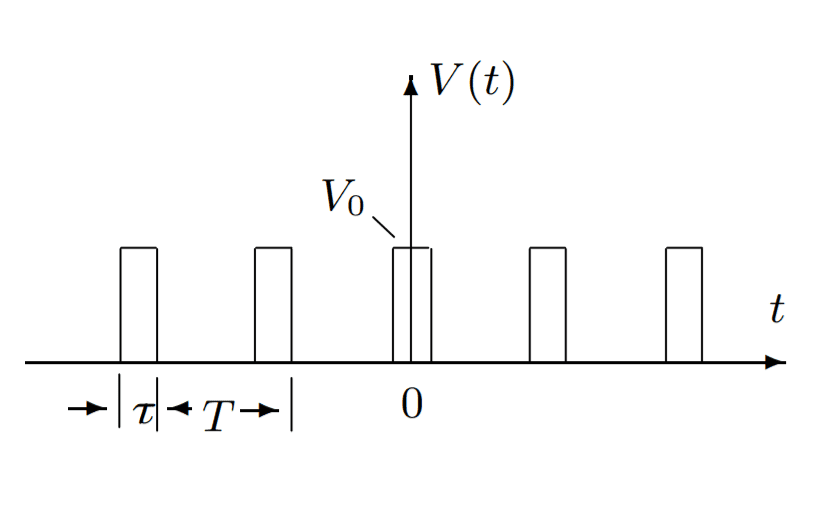
\includegraphics[width=0.9\linewidth]{img/sp1.png}}
                        \caption{Прямоугольные импульсы}
                    \end{minipage}
                    \begin{minipage}[ht]{0.45\linewidth}
                        \center{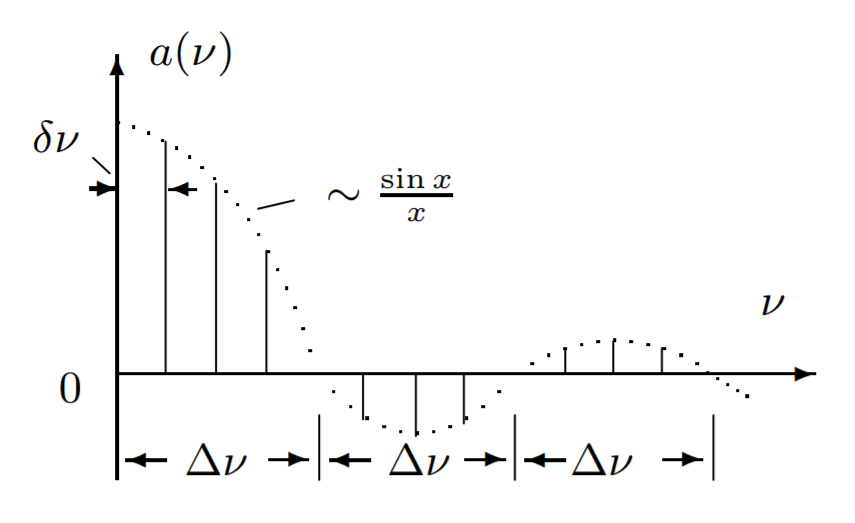
\includegraphics[width=0.9\linewidth]{img/sp2.png}}
                        \caption{Спектр последовательности прямоугольных импульсов}
                    \end{minipage}
                \end{figure}

                Назовем \textit{шириной спектра} $\Delta \omega$ расстояние от главного максимума ($\omega =0$) до первого нуля огибающей, возникающего при $n=\dfrac{2\pi}{\tau \Omega_{1}}$. При этом

                $$\Delta \omega \tau \backsimeq 2 \pi $$

                или

                \begin{equation}\label{neopr}
                    \Delta \nu \Delta t \backsimeq 1
                \end{equation}

                Полученное соотношение взаимной связи интервалов $\Delta \nu$ и $\Delta t$ является частным случаем соотношения неопределенности в квантовой механике.

            \subsubsection{Периодическая последовательность цугов}

                гармонического колебания $V_{0}\cos(\omega_{0}t)$ с длительностью цуга $\tau$ и периодом повторения $T$ (рис. 3).

                Функция $f(t)$ снова является четной относительно $t=0$. Коэффициент при $n$-й гармонике равен
                \begin{equation}
                    a_{n}=\dfrac{2}{T}\int\limits_{-\frac{\tau}{2}}^{\frac{\tau}{2}}V_{0}\cos(\omega_{0}t)\cos(n \Omega_{1} t)dt=V_{0}\dfrac{\tau}{T} \bigg(\dfrac{\sin[(\omega_{0}-n\Omega_{1})\frac{\tau}{2}]}{(\omega_{0}-n\Omega_{1})\frac{\tau}{2}}+\dfrac{\sin[(\omega_{0}+n\Omega_{1})\frac{\tau}{2}]}{(\omega_{0}+n\Omega_{1})\frac{\tau}{2}} \bigg)
                    \label{eq6}
                \end{equation}

                Зависимость для случая, когда $\frac{T}{\tau}$ равно целому числу, представлена на рис. 4. Сравнивая спектр последовательности прямоугольных импульсов и цугов мы видим, что они аналогичны, но их максимумы сдвинуты по частоте на величину $\omega_{0}$.

                \begin{figure}[ht]
                    \begin{minipage}[ht]{0.45\linewidth}
                        \center{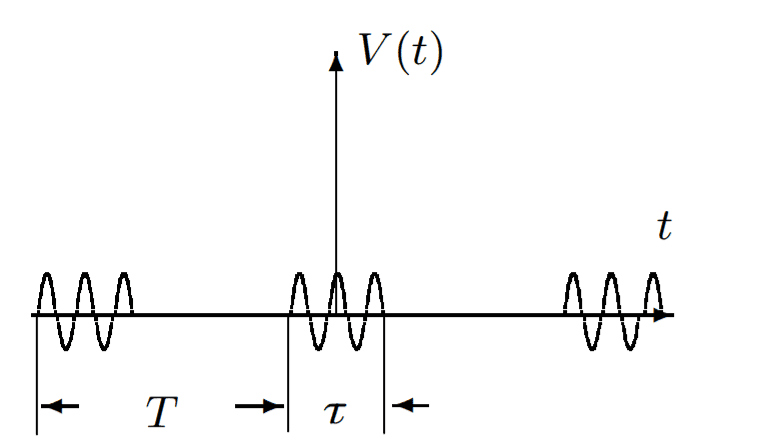
\includegraphics[width=0.9\linewidth]{img/sp3.png}}
                        \caption{Последовательность цугов}
                    \end{minipage}
                    \begin{minipage}[ht]{0.45\linewidth}
                        \center{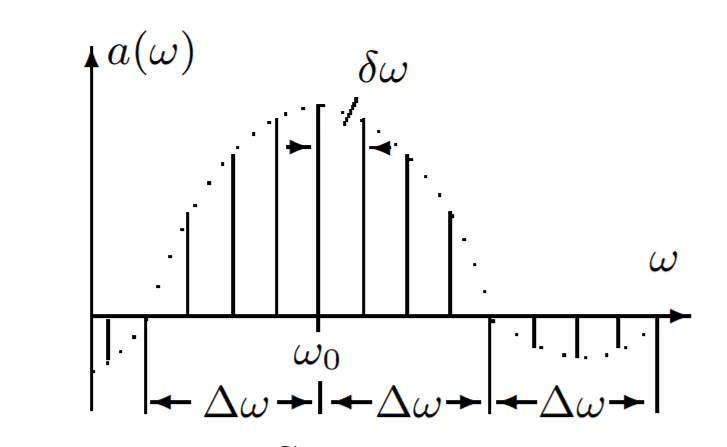
\includegraphics[width=0.9\linewidth]{img/sp4.png}}
                        \caption{Спектр последовательности цугов}
                    \end{minipage}
                \end{figure}

            \subsubsection{Амплитудно-модулированные колебания}

                Рассмотрим гармонические колебания высокой частоты $\omega_{0}$ , амплитуда которых медленно меняется по гармоническому закону с частотой $\Omega$ ($\Omega \ll \omega_{0})$) (рис. 5):
                \begin{equation}
                    f(t)=A_{0}[1+m\cos\Omega t]\cos \omega_{0}t
                    \label{eq7}
                \end{equation}

                Коэффициент $m$ называют \textbf{глубиной модуляции}. При $m<1$ амплитуда колебаний меняется от минимальной $A_{min}=A_{0}(1-m)$ до максимальной $A_{max}=A_{0}(1+m).$ Глубина модуляции может быть представлена в виде

                \begin{equation}\label{m}
                    m=\dfrac{A_{max}-A_{min}}{A_{max}+A_{min}}
                \end{equation}

                Простым тригонометрическим преобразованием можно найти спектр амплитудно - модулированных колебаний:

                \begin{equation}\label{a}
                    f(t)=A_{0}\cos(\omega_{0} t)+\dfrac{A_{0}m}{2}\cos(\omega_{0}+\Omega)t+\dfrac{A_{0}m}{2}\cos(\omega_{0}-\Omega)t.
                \end{equation}

                \begin{figure}[ht]
                    \begin{minipage}[ht]{0.45\linewidth}
                        \center{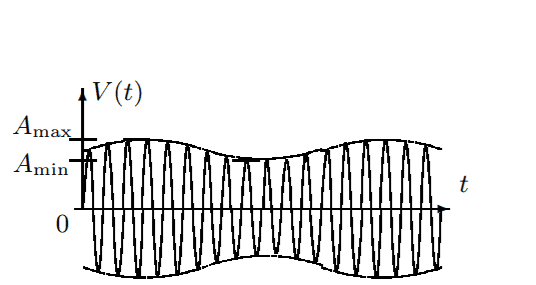
\includegraphics[width=0.9\linewidth]{img/sp5.png}}
                        \caption{Модулированные гармонические колебания}
                    \end{minipage}
                    \begin{minipage}[ht]{0.45\linewidth}
                        \center{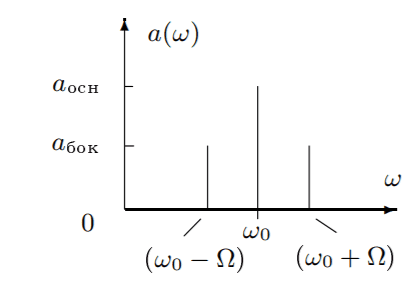
\includegraphics[width=0.9\linewidth]{img/sp6.png}}
                        \caption{Спектр модулированных гармонических колебаний}
                    \end{minipage}
                \end{figure}

                Спектр таких колебаний содержит три составляющих  основную компоненту и две боковых (рис. 6). Первое слагаемое в правой части представляет собой исходное немодулированное колебание с основной (несущей) частотой $\omega_{0}$ и амплитудой $a_{осн} = A_{0}$ . Второе и третье слагаемые соответствуют новым гармоническим колебаниям с частотами $\omega_{0} + \Omega$ и $\omega_{0} - \Omega$. Амплитуды этих двух колебаний одинаковы и составляют $\dfrac{m}{2}$ от амплитуды немодулированного колебания:

                $a_{бок} = \dfrac{A_{0}m}{2}$. Начальные фазы всех трех колебаний одинаковы.

\end{document}
